\chapter{Struktura Aplikacji}

Struktura aplikacji została częściowo opisana w rozdziale \hyperref[ch:manual]{\textbf{Podręcznik użytkownika}}.

\section{Edytor notatki}

Edytor notatki składa się z edytora tytułu znajdującego się w głównym pasku strony edycji notatki, oraz edytora zawartości.

Do zarządzania zawartością notatki używana jest klasa NoteParagraphs przechowująca listę obiektów typu NoteParagraph reprezentującymi paragrafy notatki.
Współpracę tych klas można przedstawić w uproszczony sposób za pomocą schematu:
\begin{figure}[ht]
    \centering
    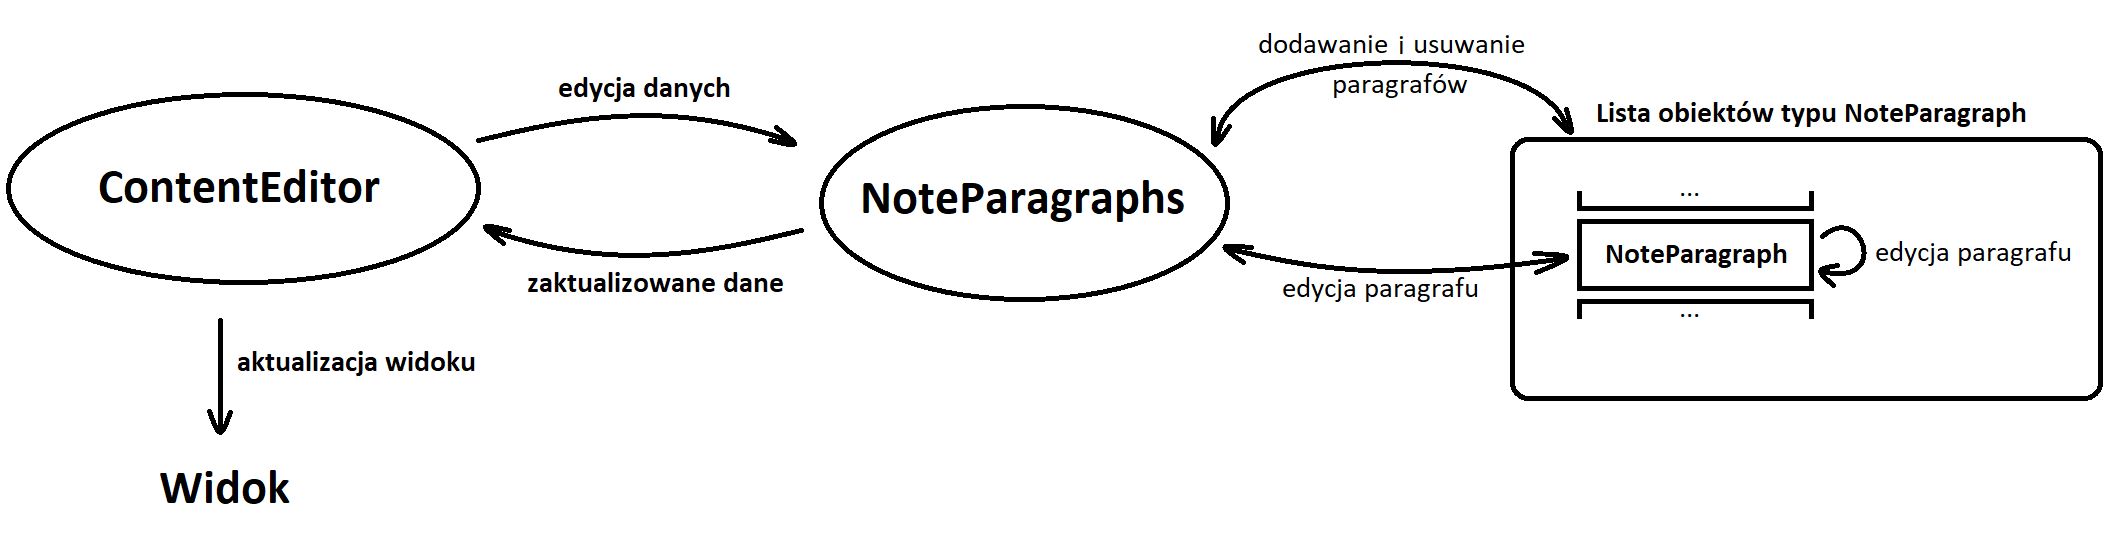
\includegraphics[width=\linewidth]{images/ContentEditor_podzial.png}
    \caption{Uproszczony schemat zarządzania paragrafami.}
\end{figure}